\documentclass[../main.tex]{subfiles}
\begin{document}
\section{Simulation}
\labsec{sim}

All the simulations were performed using open source softwares (Code Aster and OpenFOAM\sidecite{article}).
For reproducility, all the custom code used is also open sourced at \href{https://github.com/leoank/cool_chip}{https://github.com/leoank/cool\_chip}.

\subsection{Geometry}

\subsubsection{Fin profile}

Radius of cylindrical fins can be expressed as:
\begin{equation}
    r(x) = r_1 + (r_2 - r_1)(1 - \frac{x}{L})^n
\end{equation}
\\
Where, $r_1$ and $r_2$ are base and tip radius. $n$ is the concavity of the fin.
\\
Some of the generated fin profile are shown below.
\begin{figure}[H]
    \centering
    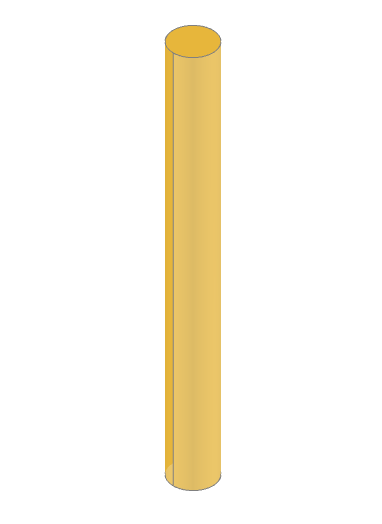
\includegraphics[height=5cm,keepaspectratio]{cy_fin_0.0.png}
    \caption{Cylindrical fin with n=0}
    \label{fig:cyfin00}
\end{figure}

\begin{figure}[H]
    \centering
    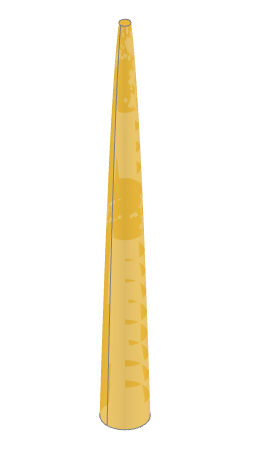
\includegraphics[height=5cm,keepaspectratio]{cy_fin_0.5.png}
    \caption{Cylindrical fin with n=0.5}
    \label{fig:cyfin05}
\end{figure}

\begin{figure}[H]
    \centering
    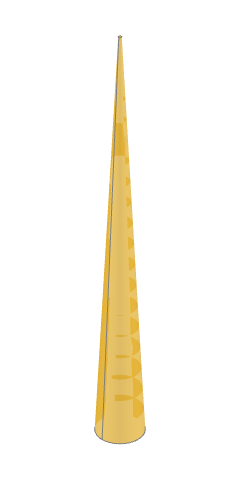
\includegraphics[height=5cm,keepaspectratio]{cy_fin_1.0.png}
    \caption{Cylindrical fin with n=1.0}
    \label{fig:cyfin10}
\end{figure}

\begin{figure}[H]
    \centering
    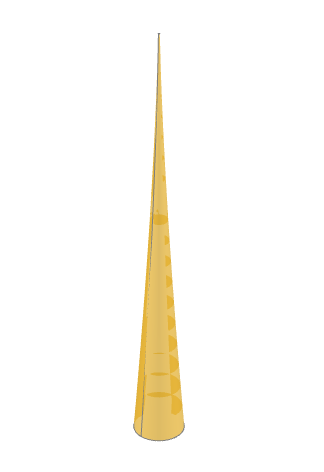
\includegraphics[height=5cm,keepaspectratio]{cy_fin_2.0.png}
    \caption{Cylindrical fin with n=2.0}
    \label{fig:cyfin20}
\end{figure}

\subsection{Governing equations}
\subsubsection{Thermal simulation}
\begin{equation}
    \rho c_p \frac{\partial T}{\partial t} + \rho c_p \frac{\partial (u T)}{\partial x}  = k \frac{\partial^2 T}{\partial x^2} + Q
\end{equation}

\subsubsection{Nanofluid simulation}

We used a two phase, Lagrangian-Eulerian model as suugested by Safaei et al.\sidecite{Safaei2016}
\\
Conservation of mass:
\begin{equation}
    \nabla (\rho u) = 0
\end{equation}
\\
Conservation of momentum:
\begin{equation}
    \nabla (\rho u u) = \nabla P + \nabla (\mu \nabla u) + S_m
\end{equation}
\\
Conservation of energy:
\begin{equation}
    \nabla(\rho c_p u T) = \nabla (k \nabla T) + S_e
\end{equation}
\\
Where, $S_m$ and $S_e$ are source/sink terms representing the exchange of momentum and energy
between liquid and solid phases.

\begin{equation}
    S_m = \frac{1}{\delta V} \sum_{np}F
\end{equation}

\begin{equation}
    S_e = \frac{1}{\delta V} \sum_{np}Nu_p \pi d_p k_p (T - T_p)
\end{equation}
\\
Where $Nu_p$ can be expressed as:
\\
\begin{equation}
    Nu_p = 2 + 0.6Re_p^{0.5} Pr^{0.33}
\end{equation}

\end{document}
